
\section[Statistics]{Statistical Interpretation of the results}\label{sect:stat}

Since no excess of data over the background prediction has been observed, 
we close our study with setting upper limits on the testing signals.
This is conducted using a modified frequentist approach, namely CLs method \cite{read:CLs}.
In this method, the test statistic $q_\mu$ \cite{cowan:asymptoticCLs} is a function of the profile likelihood-ratio,

\begin{align}
q_\mu = -2 \ln \frac{\mathcal{L}(data ;\, b + \mu s)}{\mathcal{L}(data ;\, b + \hat{\mu} s)},
\end{align}

where $\hat\mu$ is the \textit{signal strength modifier} $\mu$ at the maximum point of the likelihood $\mathcal{L}$.
Then CLs is given by the following probability-ratio,

\begin{align}
CL_s = \frac{p(q_\mu \geq q_\mu^{obs} | b + \mu s )}{p(q_\mu \geq q_\mu^{obs} | b)}.
\end{align}
 
We compute CLs using a software package provided by the CMS Higgs PAG \cite{higgspag:software}.
After incorporating systematic uncertainties, an observed CLs smaller than 0.05 for a signal strength of $\mu = 1$, excludes the given signal at $95\%$ CL. Indeed, the package determines which signal strength $\mu$ excludes the testing signal at $95\%$ CL. Therefore all resulting $\mu \leq 1$ define the excluded region in the parameter space of the given signal. 

In this study, we analyze data in 8 different bins (multi-bin analysis) to utilize more information from 
the observed and the predicted distributions.
%bins' contents of the observations and the predictions.
The bins are defined in reconstructed top quark multiplicity, zero or more. In addition, events are categorized based on the $\mttwo$ values: $125\rm{GeV} \leq \mttwo < 150\rm{GeV},\; 150\rm{GeV} \leq \mttwo < 200\rm{GeV},\; 200\rm{GeV} \leq \mttwo < 250\rm{GeV},\; 250\rm{GeV} \leq \mttwo < \infty$.
%These bins are determined, for an event, based on whether the event contents reconstructed top quarks or not (2 bins) times which bin of $\mttwo$ is occupied by the event (4 bins of $125\rm{GeV} \leq \mttwo < 150\rm{GeV},\; 150\rm{GeV} \leq \mttwo < 200\rm{GeV},\; 200\rm{GeV} \leq \mttwo < 250\rm{GeV},\; 250\rm{GeV} \leq \mttwo < \infty$). 

To investigate the exclusion power of our research, we study the topology of direct stop pair production  in Simplified Models \cite{alves:sms}, with $\tilde{t}\to \tilde{\chi}^0_1 t$ (T2tt). 
Calculation of the expected exclusion limit shows that  
the research has potential to exclude 
%excludes 
a sizable region of the phase space, surrounded by the lines of $m_{\tilde{t}} = 600\rm{GeV}$ and $m_{LSP} = 175\rm{GeV}$ with an integrated luminosity of $19.6\,\invfb$.



Figure \ref{fig:limit_20inf} shows the expected upper limit on the cross section of the stop pair production in terms of Simplified Models. 
Furthermore, the figure shows the expected exclusion power considering 
$40\%$ systematic uncertainties on signal and background rates which are predicted using Monte-Carlo simulations. The black 
dashed curve represents the expected reach by the common Cut$\&$Count \cite{cutandcountAN} search using $\met$ trigger. 
As the figure shows our analysis (the blue solid curve) can be comparable with other analyses and   
it has the potential to be complementary to other analyses in some regions of the phase space.  



%%%%%%%%%%
\begin{linenomath}
\begin{figure}[h]
\centering
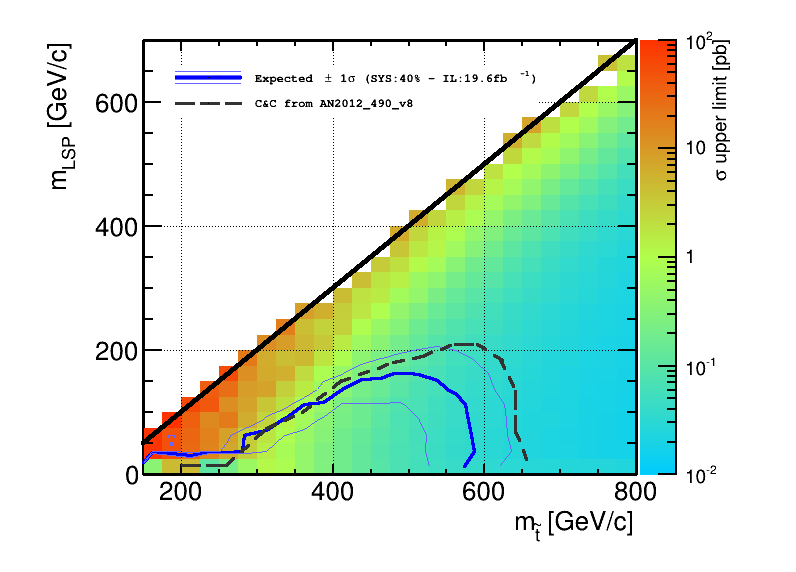
\includegraphics[width=0.9\textwidth,keepaspectratio=true]{StatisticsFig/Exc_131030_196ifb.png}
\caption{Expected exclusion power in terms of Simplified Models (T2tt-topology) with an integrated luminosity of $20\,\invfb$. Backgrounds are predicted using Monte-Carlo simulations and a rough estimate of systematic uncertainties equal 
$40\%$ is taken into account.}
\label{fig:limit_20inf}
\end{figure}
\end{linenomath}
%%%%%%%%%%


%%%%%%%%%%
%\begin{linenomath}
%\begin{figure}[h]
%\centering
%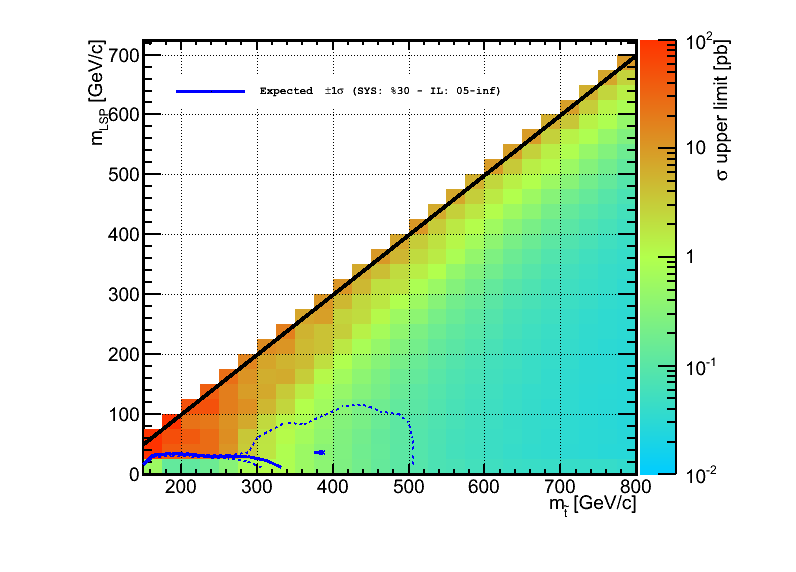
\includegraphics[width=0.7\textwidth,keepaspectratio=true]{StatisticsFig/limit_30sys_05inf_20130625.png}
%\caption{}
%\label{fig:limit_05inf}
%\end{figure}
%\end{linenomath}
%%%%%%%%%%

%%%%%%%%%%
%\begin{linenomath}
%\begin{figure}[h]
%\centering
%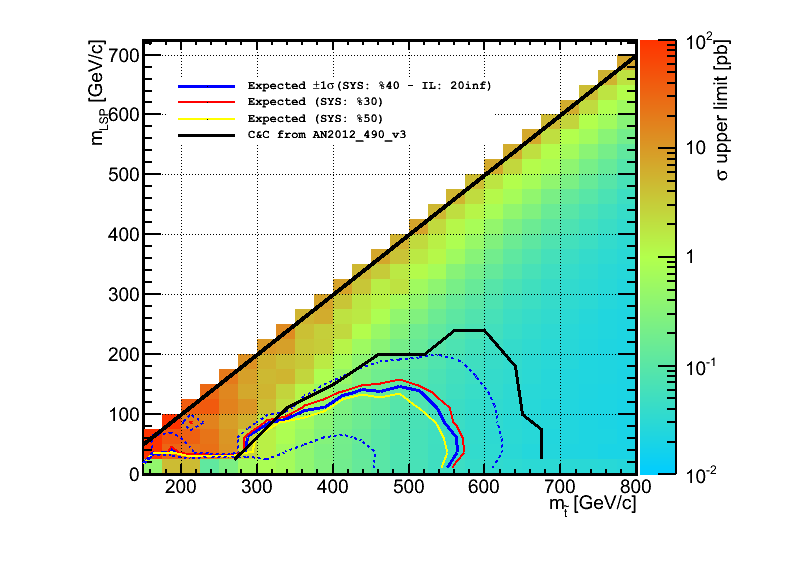
\includegraphics[width=0.7\textwidth,keepaspectratio=true]{StatisticsFig/limit_304050sys_20inf_20130625.png}
%\caption{}
%\label{fig:limit_20inf}
%\end{figure}
%\end{linenomath}
%%%%%%%%%%

